\newpage
\section{Entwicklung}
In diesem Kapitel wird die schrittweise Entwicklung des digitalen Zwillings der robocell beschrieben.
Zunäscht werden alle relevanten Datenquellen identifiziert und geeignete Submodelle der \acs{aas} ausgewählt.
Darauf aufbauend folgt die Modellierung dieser mithilfe des Package Explorers sowie die Validierung mit einer Test Engine.
Im Anschluss wird gezeigt, wie die \acs{aas} mithilfe von Eclipse BaSyx bereitgestelllt und verwaltet werden kann.
Dabei werden sowohl Echtzeidaten über \acs{opcua} als auch Zeitreihendaten über eine InfluxDB eingebunden.
Darüber hinaus wird auf die Entwicklung von drei exemplarischen Anwendungsfällen eingegangen.
Dazu zählt unter anderem der digitale Produktpass, die automatisierte Generierung der \acs{aas} sowie der Einsatz von \acs{ki}.

\subsection{Konzeptionierung des digitalen Zwilling}
Ziel dieses Abschnittes ist es, eine grundlegende Basis für die Erstellung des digitalen Zwillings zu schaffen.
Dabei wird untersucht, welche Daten für die Modellierung erforderlich sind, wo diese herkommen und wie sie in (standardisierten) Teilmodellen der \acs{aas} strukturiert werden können.
\subsubsection{Identifikation relevanter Datenquellen}
Ein digitaler Zwilling basiert immmer auf einer Vielzahl unterschiedlicher Daten, die gemeinsam ein umfassendes digitales Abbild eines Assets ermöglichen. 
Dabei werden sowohl statische Informationen (z.B. Datenblätter oder Konstruktionsdaten) als auch dynamische Daten, die während des Betriebs einer Maschine anfallen, benötigt.
Im ersten Schritt gilt es daher, alle relevanten Datenquellen zu identifizieren, die für die Modellierung des digitalen Zwillings erforderlich sind.

In industriellen Umgebungen kommen typischerweise verschiedene Systeme zur Erfassung, Verwaltung und Speicherung von Maschinendaten zum Einsatz.
Bei groninger übernimmt diese Funktion das \acs{plm}-System Agile, das eng mit dem \acs{erp}-System PSI Penta verknüpft ist.
Darin sind unter anderem Stücklisten, technische Spezifikationen, \acs{cad}-Dateien sowie allgemeine Dokumente hinterlegt, die die statische Grundlage  für den digitalen Zwilling bilden.

Neben den Informationen aus den Unternehmenssystemen spielen aber auch Laufzeitdaten, wie sie durch Sensoren oder Steuerungssysteme erzeugt werden, eine zentrale Rolle.
Da im Rahmen dieser Arbeit keine reale Maschine angebunden ist, werden diese Daten simuliert.
Hierfür kommt eine in Node.js entwickelte Anwendung zum Einsatz, die im Folgenden als Datengenerator bezeichnet wird und sowohl Prozess- als auch Betriebsdaten generiert. 
Ergänzend dazu wird ein Maschinensimulator verwendet, der einen PackML-Zustandsautomaten abbildet und typische Maschinenzustände sowie deren Übergänge simuliert. 
Beide Komponenten stehen als Docker Container zur Verfügung und stellen die Daten über einen \acs{opcua} Server bereit, wodurch eine realitätsnahe Datenbasis geschaffen wird.
\subsubsection{Auswahl geeigneter Teilmodelle}
Aufbauend auf den zuvor betrachteten Informationsquellen gilt es nun zu entscheiden, welche Aspekte der Maschine im digitalen Zwilling, oder besser gesagt in der \acs{aas}, abgebildet werden sollen.
Im nächsten Schritt ist daher die Auswahl bzw. der Entwurf geeigneter Submodelle erforderlich, die die relevanten Informationen strukturiert bereitstellen.

Als Orientierung dienen die von der \acs{idta} bereitgestellten Submodel Templates \cite{idtaTemplates}, die bereits viele typische Anwendungsfälle standardisiert abdecken.
Diese sind jeweils in einer Submodellspezifikation der \acs{idta} dokumentiert.
Darüber hinaus besteht jedoch auch die Möglichkeit, eigene Submodelle zu entwerfen, die gezielt auf projektspezifische Anforderungen zugeschnitten sind.
Diese können entweder vollständig neu konzipiert oder aus bestehenden Vorlagen abgeleitet werden.

Die konkrete Auswahl der Submodelle in dieser Arbeit orientiert sich hauptsächlich an typischen Industrie 4.0-Anwendungsfällen, die unter anderem auf der Website der \acs{idta} dokumentiert sind \cite{idtaUseCases}.
Diese Anwendungsfälle zeigen auf, welche Submodelle in der Praxis besonders relevant sind.
Eines der wichtigsten ist vermutlich das digitale Typenschild, da dieses häufig die erste Anlaufstelle für die Identifikation und grundlegende Informationen eines Assets darstellt.
Daneben wurden aber auch projektspezifische Anforderungen berücksichtigt, die sich aus den verfügbaren Daten sowie dem fachlichen Austausch mit Industriepartnern wie Wittenstein ergaben.

Tabelle \ref{tab:Submodelle} liefert einen Überblick über die initiale Auswahl dieser Submodelle.
In der Spalte Standardisierung ist jeweils das zugehörige Submodel Template durch die zugehörige Dokumentennumer der \acs{idta} angegeben, in der die entsprechende Version dokumentiert ist.
Die in der Spalte Vorgesehene Inhalte genannten Punkte zeigen beispielhaft auf, welche Informationen im digitalen Zwilling abgebildet werden sollen.

Diese Submodelle werden in späteren Anwendungsfällen gezielt erweitert.
Ein wesentlicher Vorteil der \acs{aas} besteht nämlich in ihrer Flexibilität.
Submodelle können sukszessive ergänzt, angepasst oder auch wieder entfernt werden, ohne dabei die bestehende Struktur des digitalen Zwillings zu verändern.
% Wie erfolgt die Auswahl? sss

%Nachfolgende Tabelle gibt einen Überblick über die wichtigsten, in diesem Projekt eingesetzten Submodelle sowie ihrer Inhalte.
%Die bereits veröffentlichten Modelle sind dabei jeweils in einer Spezifikation der \acs{idta} standardisiert.

%\newpage
{\small
\begin{longtblr}[
    label = tab:Submodelle,
    entry = Submodelle mit typischen Inhalten,
    caption = {Submodelle mit typischen Inhalten}
  ]{
    colspec = {l l X[c]},
    rowhead = 1,
    vlines,
    hline{1-11} = {-}{},
    }
    \textbf{Submodell}                                   & \textbf{Typische Inhalte}                            & \textbf{Standardisierung} \\
    Typenschild                                          & \makecell[l]{Hersteller \\ Seriennummer \\ Adressinformationen}                  & IDTA 02006-3-0 \cite{SpezifikationTypenschild} \\
    Dokumentation                                     & \makecell[l]{Allgemeine Dokumente \\ Betriebsanleitungen \\ Projektzeichnungen}             & IDTA 02004-1-2 \cite{SpezifikationDokumentation} \\
    3D-Modelle                                           & Konstruktionsmodelle                & IDTA 02026-1-0 \cite{Spezifikation3DModelle}\\*
    Technische Daten                                     & \makecell[l]{Generelle Informationen \\ Technische Eigenschaften }                       & IDTA 02003 \cite{SpezifikaitonTechnischeDaten}\\*
    \acs{bom}                                     &  \makecell[l]{Strukturierte Stücklisten \\ Komponentenbeziehungen }                    & IDTA 02011-1-1 \cite{SpezifikationHierachischeStrukturen}\\*
    Wartung                                              &  \makecell[l]{Wartungsinformationen \\ Wartungsintervalle \\ }          & -  \\*
    Prozessdaten                                         &  \makecell[l]{Messwerte}             & - \\*
    Zeitreihendaten                                       &  \makecell[l]{Zeitreihen }             & IDTA 02008-1-1 \cite{SpezifikationTimeSeriesData}    \\*
    Kontrollkomponente                                   &  \makecell[l]{Betriebsmodi \\ Schnitstelle zur Automatisierung }             & - \\      
\end{longtblr}
}

Ein besonders wichtiges Submodell stellt die Stückliste (\acs{bom}) dar.
Mit diesem lässt sich die hierarchische Struktur eines Assets abbilden, das aus mehreren verschachtelten Komponenten besteht.
Für komplexe Maschinen oder Anlagen, wie im Fall der robocell, wird im Rahmen dieser Konzeption vorgesehen, einzelne Komponenten jeweils als eigene \acs{aas}-Instanzen zu modellieren und in der übergeordneten Haupt-\acs{aas} zu referenzieren.
Auf diese Weise soll eine höhere Modularität und Wiederverwendbarkeit erreicht werden.

Zur Verdeutlichung der zugrunde liegenden Architektur sowie der Beziehungen zwischen den identifizierten Datenquellen, \acs{aas} und Submodellen dient Abbildung~\ref{fig:konzeptionierungAAS}. 
Die \acs{aas} der robocell bildet dabei das zentrale digitale Abbild, in das die relevanten Informationen aus den in diesem Kapitel beschriebenen Submodellen integriert werden sollen.

Einzelne Maschinenkomponenten werden durch eigene Komponenten-\acs{aas} repräsentiert. 
In der Abbildung sind exemplarisch zwei Industrie-4.0-Komponenten der ersten Ebene der Komponentenstruktur dargestellt. 
Weitere, hierarchisch untergeordnete Bauteile oder Baugruppen können analog ebenfalls als eigenständige \acs{aas}-Instanzen modelliert und über entsprechende Referenzen in die Haupt-\acs{aas} der robocell oder in übergeordnete Strukturen eingebunden werden.

\begin{figure}[htbp]
    \centering
    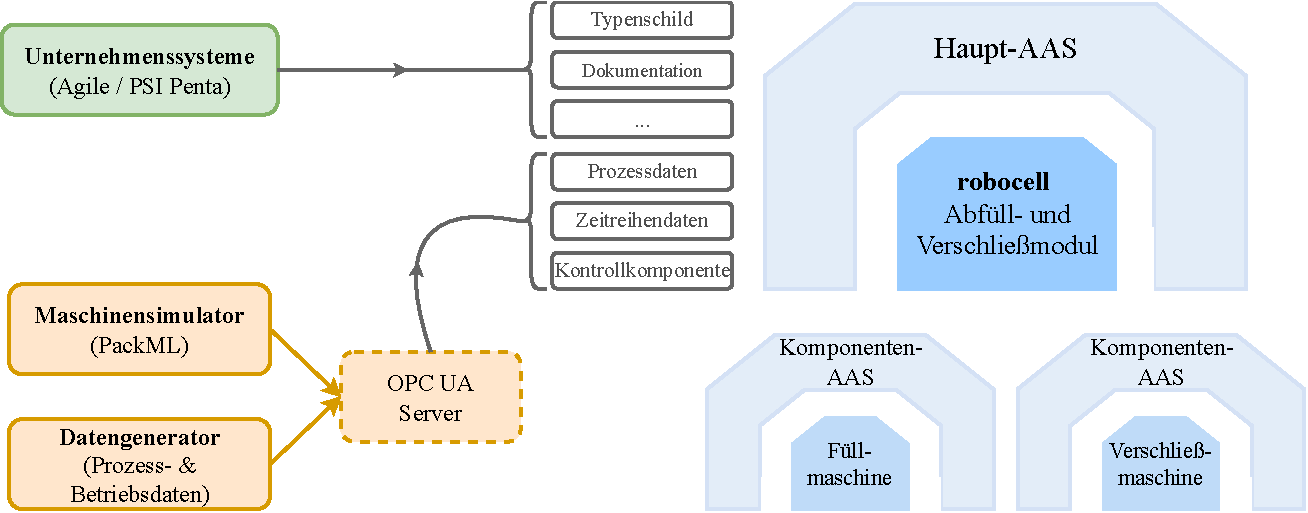
\includegraphics[width=1\textwidth]{Bilder/Konzeptionierung/konzeptionierung.pdf}
    \caption{\acs{aas}-Konzept der robocell}
    \label{fig:konzeptionierungAAS}
\end{figure}

\subsection{Modellierung mit der AAS}

In diesem Abschnitt wird erläutert, wie die zuvor ausgewählten Submodelle in eine \acs{aas} integriert und mit konkreten Daten befüllt werden können.
Die Modellierung erfolgt dabei mithilfe des Package Explorers.
Außerdem wird gezeigt, wie sich die erstellte \acs{aas} mit einer Test Engine auf eine korrekte und vollständige Struktur überprüfen lässt.

\subsubsection{Umsetzung mit dem Package Explorer}
Für die manuelle Erstellung der \acs{aas} kann der Package Explorer eingesetzt werden.
Dieser erlaubt eine eine intuitive Modellierung aller relevanten Elemente einer \acs{aas} und erleichtert so den strukturierten Aufbau des digitalen Zwillings.

Zunächst muss ein neues \acs{aas}-Paket erstellt werden.
Hierzu kann im Package Exporer eine neue Umgebung geöffnet werden, die als Container für die Inhalte eines Assets dient.
Anschließend lässt sich eine neue \acs{aas} anlegen, die allgemeine Informationen sowie assetspezifische Daten beeinhaltet.

Neben der Auswahl des Asset-Typs (Instanz oder Typ) ist insbesondere die eindeutige Identifikation von zentraler Bedeutung.
Das Asset selbst wird über eine globalAssetId referenziert, während die \acs{aas} eine eigene ID sowie eine idShort erhält.
Für erste Modellierungszwecke empfiehlt es sich, Beispiel-IDs zu verwenden, die direkt im Package Explorer generiert werden können.
Diese erleichtert nicht nur den späteren Austausch der \acs{aas}, sondern auch deren systemweites Auffinden innerhalb eines Industrie 4.0-Ökosystems.
% Darüber hinaus besteht ebenfalls die Möglichkeit, ein Thumbmail in Form einer Datei (z.B. png oder jpeg) zu hinterlegen.

Im nächsten Schritt müssen die benötigten Submodelle hinzugefügt werden. Auch diese lassen sich entweder als Instanz oder Typ anlegen.
Dabei besteht die Möglichkeit, entweder ein leeres Submodell manuell mit verschiedenen Submodellelementen zu erstellen oder auf ein vorhandenes Submodel Template zurückzugreifen.
Letztere können als AASX-Datei, beispielsweise über das Repository der \acs{idta} \cite{idtaTemplates}, heruntergeladen und anschließend über ein sogenanntes Auxiliary AAS in die Umgebung geladen werden.
Anschließend müssen die in den Submodellen enthaltenen Elemente mit konkreten Inhalten wie Werten, Dateien, Referenzen oder Beziehungen gefüllt werden.

Für die Abbildung hierarchischer Strukturen, insbesondere im Submodell \acs{bom}, kommen verschiedene Entitäten zum Einsatz.
Diese repräsentieren einzelne Komponenten bzw. Baugruppen eines Produkts.
Bei komplexeren Maschinen oder Anlagen, wie im Fall der robocell, ist es sinnvoll, solche Komponenten als eigenständige \acs{aas} zu modellieren.
Diese können dann im Package Explorer als SelfManagedEntity angelegt und über ihre globalAssetId referenziert werden, wodurch eine klare Trennung zwischen der Haupt-\acs{aas} sowie den referenzierten Kompnenten-\acs{aas} erfolgt.

Besonders bei der Verwendung von Templates muss darauf geachtet werden, dass die Struktur dieser nicht verändert wird, da dies sonst zu Abweichungen von der Submodellspezifikation führen kann.
Eine Übersicht über die Modellierungsumgebung im Package Explorer mit einem geöffneten Submodell ist in Abbildung \ref{fig:BearbeitungsansichtPackageExplorer} dargestellt.

\begin{figure}[htbp]
    \centering
    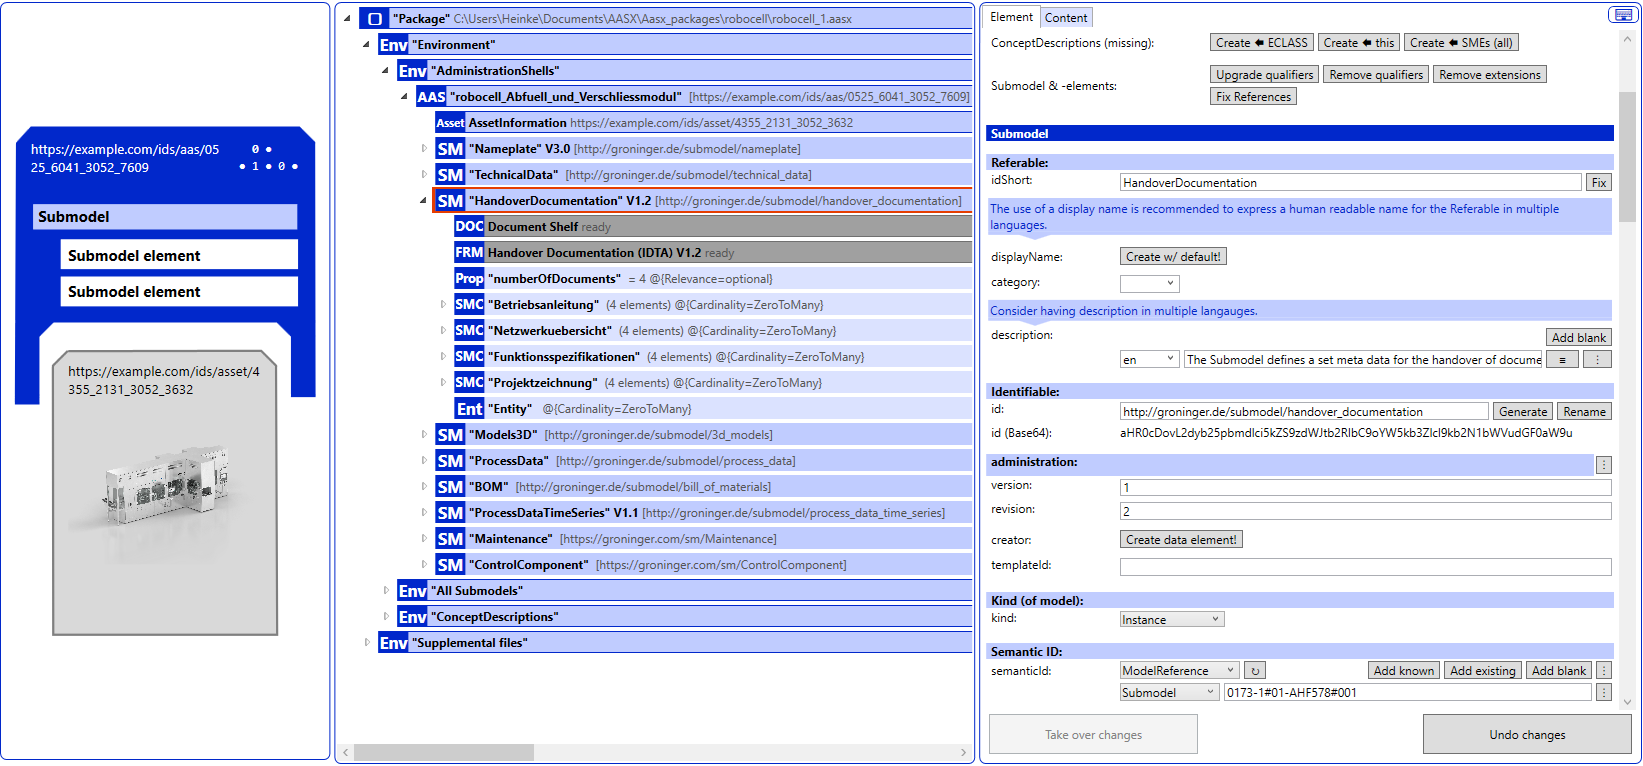
\includegraphics[width=1\textwidth]{Bilder/ModellierungAAS/ModellierungMitDokumentation.PNG}
    \caption{Bearbeitungsansicht eines Submodells im Package Explorer}
    \label{fig:BearbeitungsansichtPackageExplorer}
\end{figure}

Wie auch in der Abbildung zu erkennen, kann jedem Submodell bzw. jedem Submodellellement eine semanticId zugewiesen werden.
Diese dient der einheitlichen semantischen Beschreibung und verweist entweder auf externe Standards wie ECLASS oder auf lokale Concept Descriptions innerhalb der AAS-Umgebung.
Der Package Explorer bietet hierfür eine erweiterte Funktion, bei der sich vorgefertigte ECLASS-Kataloge importieren lassen.
Die darin enthalten Begriffe können direkt im Package Explorer dursucht, ausgewählt und den enstprechenden Submodellen bzw. Submodellelementen zugewiesen werden.

Sobald alle gewünschten Submodelle mit Inhalten gefüllt und semantisch beschrieben sind, muss die \acs{aas} gespeichert und exportiert werden.
In diesem Projekt erfolgt dies bevorzugt im AASX-Format, das sich als standardisierte Austauschform für die \acs{aas} etabliert hat und eine einfache Weitergabe ermöglicht.


\subsubsection{Validierung}
Im Anschluss an die Erstellung der \acs{aas} sollte eine Überprüfung der Konformität erfolgen.
Hierzu kann eine von der \acs{idta} bereitgestellte Test Engine \cite{TestEngine} eingesetzt werden. 
Diese lässt sich direkt mit pip, dem Paktemanager von Python, installieren und anschließend über die Kommandozeile nutzen.
Mit dem Befehl \verb|aas_test_engines check_files robocell.aasx| kann beispielsweise die Validierung der zuvor erstellten AASX-Datei der robocell gestartet werden.

%Mit dem Befehl: aas_test_engines check_file my_aas.aasx kann eine AASX-Datei validiert werden.
% \begin{verbatim}
% aas_test_engines check_file robocell.aasx
% \end{verbatim}
Dabei wird zunächst geprüft, ob die AASX-Datei formal korrekt aufgebaut ist, insbesondere hinsichtlich der internen Struktur und ihrer Beziehungen.
Anschließend erfolgt die Kontrolle der enthaltenen \acs{aas} gegen die Metamodell-Spezifikationen der \acs{idta} (Teil 1 \cite{SpezifikationPart1} und 3a \cite{SpezifikationPart3a}).
Zuletzt erfolgt ein Abgleich der Submodelle mit den zugehörigen Templates, sofern diese für das jeweilige Submodell definiert wurden.

Treten bei der Validierung formale oder semantische Fehler auf, beispielsweise durch fehlende Referenzen oder ungültige IDs, gibt die Test Engine eine detaillierte Fehlermeldung in der Konsole aus. 
Diese Hinweise geben Aufschluss darüber, an welcher Stelle die Struktur bzw. der Inhalt der AASX-Datei fehlerhaft ist, und ermöglichen so eine gezielte Korrektur der betroffenen Elemente. 
Werden im gesamten Prüfprozess hingegen keine Fehler oder Abweichungen festgestellt, bestätigt die Test Engine die erfolgreiche Validierung.
%(siehe Abbildung \ref{fig:KonsolenausgabeTestEngine}).
% \setlength{\fboxsep}{0pt}
% \begin{figure}[htbp]
%     \centering
%     \fcolorbox{black!60}{white}{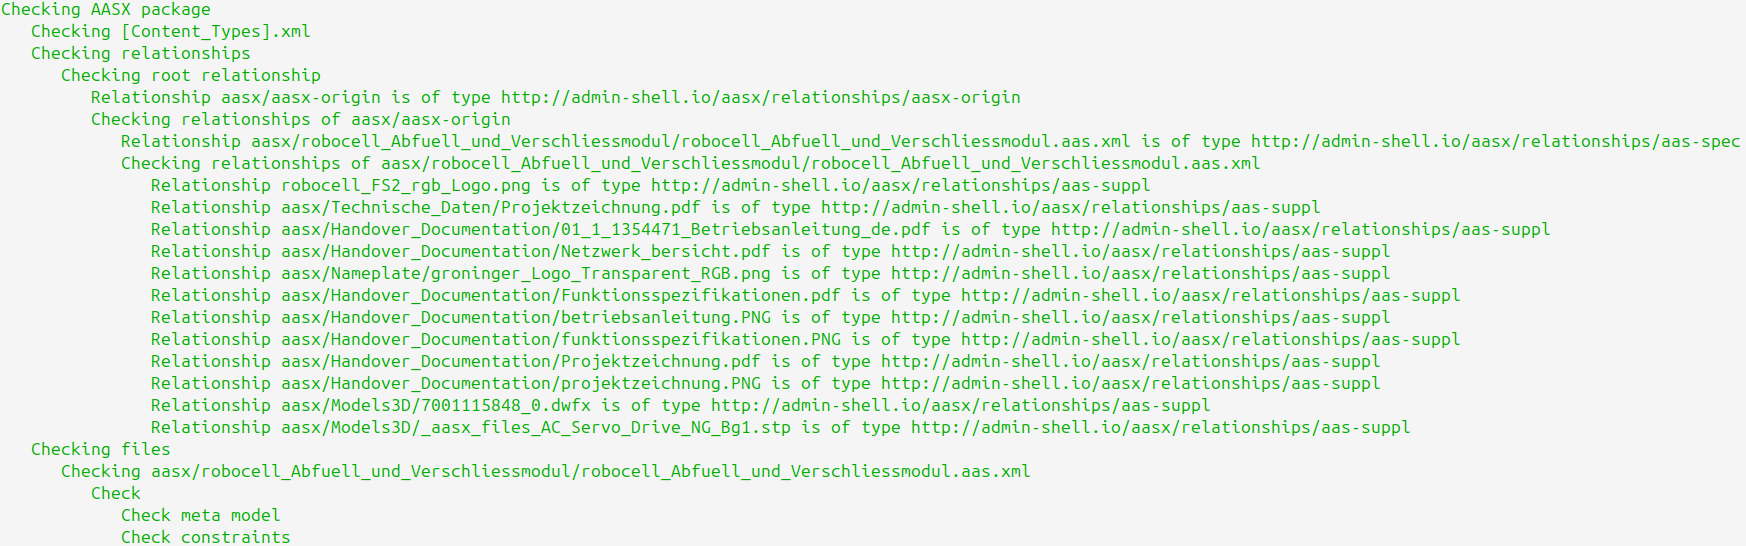
\includegraphics[width=0.99\textwidth]{Bilder/testEngineSuccess.PNG}}
%     \caption{Konsolenausgabe nach erfolgreicher Validierung}
%     \label{fig:KonsolenausgabeTestEngine}
% \end{figure}

\subsection{Technische Integration}
Im Anschluss an die Konzeption und Modellierung des digitalen Zwillings liegt der Fokus dieses Kapitels auf der technischen Integration der zuvor erstellten \acs{aas} in eine Industrie 4.0-kompatible Umgebung. 
Mithilfe der Eclipse BaSyx-Plattform wird gezeigt, wie die statisch modellierte \acs{aas} in eine Typ-2-\acs{aas} überführt und systemseitig bereitgestellt werden kann. 
Darüber hinaus wird die Erweiterung um dynamische Informationen anhand der Anbindung von Echtzeit- und Zeitreihendaten über standardisierte Schnittstellen erläutert.

\subsubsection{Bereitstellung der \acs{aas}}
\label{sec:bereitstellungAAS}
Für die Bereitstellung der \acs{aas} stehen mehrere Open-Source-Lösungen zur Verfügung. 
Eine Lösung, die sich besonders gut für den Einstieg eignet, ist der AasxServerBlazor \cite{AASXServer}, der das serverseitige Gegenstück zum Package Explorer bildet. 
Diese Kombination ermöglicht eine einfache Visualisierung sowie Verwaltung von \acs{aas}-Paketen und ist vorallem für erste Tests hilfreich.

Für komplexerer Anwendungsfälle erweist sich der AasxServerBlazor jedoch als nicht optimal, insbesondere im Hinblick auf die Integration von Echtzeitdaten sowie die dynamische Erweibarkeit von Submodellen.
Aus diesem Grund wird im weiteren Verlauf dieses Projekts die Eclipse BaSyx-Plattform eingesetzt.
Durch ihre modulare Architektur und die klare Trennung verschiedener Komponenten wie den Registries oder den Repositories bietet sie eine deutlich flexiblere Grundlage für die Umsetzung praxisnaher Industrie 4.0-Szenarien.

Die einfachste Möglichkeit, um BaSyx zu installieren, ist über Docker.
Alle benötigten Komponenten stehen hierfür als vorgefertigtes Image öffentlich über den Docker Hub zur Verfügung.
Alternativ kann auch der Source Code von Github bezogen werden, um einzelne Kompnenten individuell anzupassen oder zu erweitern.
Die verschiedenen Services, darunter die \acs{aas} Environment, Registries für \acs{aas} und Submodelle, der Discovery Service, sowie die MongoDB als persistenter Speicher, können alle in einer zentralen docker-compose.yml Datei verwaltet werden.
Die Konfiguration erfolgt in der Regel über Umgebungsvariablen oder seperate Konfigurationsdateien, die in der docker-compose.yml referenziert werden.
Schließlich können alle Komponenten gemeinsam mit dem Befehl docker compose up gestartet werden.

Nach erfolgreichem Start der BaSyx Umgebung, gibt es mehrere Möglichkeiten, eine \acs{aas} bereitzustellen und zu registrieren.
Eine besonders einfache Variante besteht darin, dass die AASX-Datei in ein gemountedes Volume der AAS Environment abgelegt wird.
Bei einem erneuten Start der Anwendung wird diese Datei automatisch erkannt, registriert und in das BaSyx System eingebunden.
Die dabei erzeugten Daten, darunter Informationen zu \acs{aas}, Submodellen, Concept Descriptions sowie Registrierungsdaten, werden in verschiedenen Tabellen der angebunden MongoDB gespeichert.
Dies gewährleistet, dass alle relevanten Daten auch bei einem Neustart der Docker Container erhalten bleiben.

Alternativ kann die Bereitstellung auch direkt über die AAS Web Ui erfolgen.
Über die Benutzeroberfläche kann eine AASX-Datei manuell importiert werden, wodurch sie direkt im laufenden System registriert un eingebunden wird.
Diese Methode eignet sich besonders gut für Tests oder kleinere Anpassungen, da eine \acs{aas} auf diese Weise schnell und ohne direkten Zugriff auf das zugrunde liegende Dateisystem eingebunden werden kann.

Die flexibelste aber technisch anspruchsvollste Möglichkeit ist die manuelle Registrierung über die REST-API. 
Dabei kann nicht einfach eine AASX-Datei hochgeladen werden, sondern es müssen die \acs{aas}, ihre Submodelle sowie ihre Beziehungen eigenständig über die bereitgestellte Schnittstellen angelegt werden.
Dies erfolgt über JSON-Datenstrukturen, die im Body der jeweiligen Anfrage übermittelt werden.
Ein typischer Ablauf mit den zugehörigen REST-Endpunkten ist in Tabelle \ref{tab:BereitstellungInBaSyx} dargestellt.
Die Endpunkte gehören dabei zu verschiedenen Services innerhalb der AAS Environment.

{\small
\begin{longtblr}[
  label = tab:BereitstellungInBaSyx,
  caption = {Bereitstellung einer AAS über die REST-API},
  entry = Bereitstellung einer AAS über die REST-API
]{
  colspec = {l l X},
  rowhead = 1,
  vlines,
  hlines,
  row{1} = {bg=tableHeader}
}
\textbf{Schritt} & \textbf{Service} & \textbf{Endpunkte} \\
1. AAS erstellen & AAS Repository & \texttt{/shells}\\
2. Submodell(e) erstellen & Submodel Repository & \texttt{/submodels}\\
\makecell[l]{3. Submodell(e) mit \\ \acs{aas} verknüpfen} & AAS Repository & \texttt{\makecell[l]{/shells/{\{aasIdentifier\}} \\ /submodel-refs}}\\
4. \acs{cd} anlegen & \acs{cd} Repository & \texttt{/concept-descriptions}\\
\end{longtblr}
}
% Das passt evtl nicht so ganz oder überflüssig von daher vlt weglassen
% \subsubsection{Datenzugriff über standardisierte Schnittstellen}

Darüber hinaus besteht ebenfalls die Möglichkeit, eine \acs{aas} im Discovery Service zu registrieren.
Über einen sogenannten assetLink kann diese dabei logisch mit einem Asset verknüpft werden.
Die Registrierung erfolgt analog zur AAS Environment über einen REST-Endpunkt.
Besonders bei der Darstellung von hierarchischen Strukturen, etwa einer \acs{bom} mit mehreren verschachtelten Assets, hilft der Discovery Service bei der eindeutigen Zuordnung der jeweiligen \acs{aas} zu ihrem physischen Gegenstück.

\subsubsection{Integration von Echtzeitdaten über OPC UA}
Nach der Erstellung der statischen \acs{aas} der robocell und der Integration in das BaSyx-System gilt es nun, diese um dynamische Informationen zu erweitern.
Diese sind essenziell, um den aktuellen Zustand einer Maschine abbilden zu können.
Die Datenbasis bilden die beiden zuvor vorgestellten Anwendungen, die Maschinen- bzw. Sensordaten über einen \acs{opcua} Server bereitstellen.
% Auf die konkrete Simulation dieser Daten soll in dieser Arbeit allerdings nicht weiter eingegangen werden.

% Dennoch ist es sinnvoll, einmal die Struktur der bereitgestellten Daten zu betrachten.

% Zur Analyse kann ein OPC UA Client genutzt werden, z.B. UA Expert, mit dem alle verfügbaren Datenpunkte (Nodes) eingesehen werden können.
% Die Daten werden in einer hierarchischen Struktur bereitgestellt, wie sie in Abbildung \ref{fig:opcua_serverstruktur} zu erkennen ist.
% Jede Node besitzt dabei einen NamespaceIndex sowie eine eindeutige NodeId (siehe Abbildung \ref{fig:opcua_pressure_node}), über die das jeweilige Objekt identifiziert werden kann.

% \begin{figure}[htbp]
%     \centering
%     \begin{minipage}[t]{0.25\textwidth}
%         \centering
%         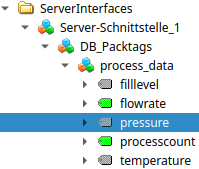
\includegraphics[width=\textwidth]{Bilder/OPCUA/serverstruktur.png}
%         \caption{OPC UA Serverstruktur}
%         \label{fig:opcua_serverstruktur}
%     \end{minipage}
%     \hspace{0.2\textwidth} % Abstand zwischen den Bildern
%     \begin{minipage}[t]{0.4\textwidth}
%         \centering
%         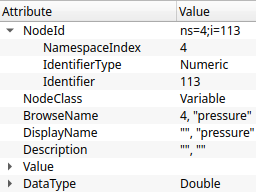
\includegraphics[width=\textwidth]{Bilder/OPCUA/pressure_node.png}
%         \caption{Detailansicht der Node \texttt{pressure}}
%         \label{fig:opcua_pressure_node}
%     \end{minipage}
% \end{figure}

Die Integration von Echtzeidaten in die \acs{aas} wird im Folgenden am Beispiel des Submodells Prozessdaten erläutert.
Innerhalb dieses Submodells existieren verschiedene Properties, die jeweils bestimmte Werte, wie beispielsweise den Druck oder die Anzahl abefüllter Einheiten, repräsentieren. %(siehe Abbildung \ref{fig:UMLSubmodellProcessData}). 
Diese Properties sollen im weiteren Verlauf dynamisch mit den simulierten Werten, die über \acs{opcua} bereitgestellt werden, aktualisiert werden.

%\begin{figure}[htbp]
%    \centering
%    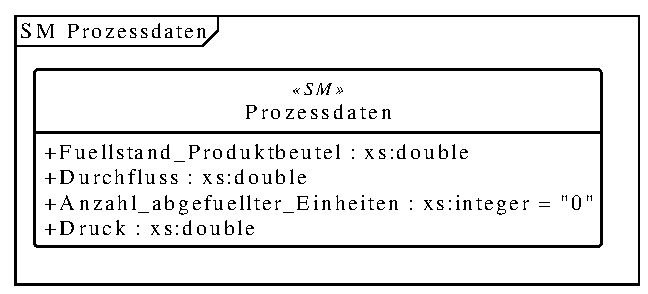
\includegraphics[width=0.6\textwidth]{Bilder/UML/submodel_processdata.pdf}
%   \caption{Klassendiagramm des Submodells Prozessdaten}
%    \label{fig:UMLSubmodellProcessData}
%\end{figure}


Das Eclipse BaSyx-Projekt stellt hierfür eine weitere Komponente bereit, die sogenannte Databridge \cite{BaSyxDatabridge}.
Diese steht, wie alle anderen Komponenten auch, als Docker Container zur Verfügung und ermöglicht die Anbindung verschiedenster Datenquellen an eine \acs{aas}.
Sie unterstützt eine Vielzahl von Protokollen, darunter insbesondere auch \acs{opcua} oder MQTT.
Dabei dient sie als Vermittler zwischen einem Datenendpunkt und einem Submodell innerhalb der \acs{aas}.

Die Konfiguration der Databridge erfolgt über mehrere JSON-Dateien.
In einer zentralen Konfigurationsdatei werden sowohl die Datenquelle als auch die Datensenke definiert.
Die Aktualisierung der Daten erfolgt dabei ereignisbasiert anhand eines Event-Triggers.

Als Datenquelle muss der \acs{opcua} Server des Datengenerators angegeben werden, dessen Konfiguration typischerweise in einer separaten JSON-Datei erfolgt.
Darin sind sowohl die Verbindungsparameter des Servers (z.B. URL und Port) als auch die zu überwachenden Knoten anzugeben.
Der \acs{opcua} Server stellt die Werte hierfür in einer hierarchischen Struktur bereit, wobei jeder Knoten über einen Namespaceindex (ns) und eine NodeId (i) eindeutig adressierbar ist.

Darüber hinaus muss der zu verwendende \acs{opcua} Client festgelegt werden.
In diesem Projekt wird Eclipse Milo eingesetzt, der auf einem Subscription-Modell basiert.
Im Gegensatz zu einem Polling-Ansatz werden hier gezielt bestimmte Knoten (Nodes) abonniert, sodass neue Werte automatisch bei Änderung übermittelt werden.

Ein Beispiel für die JSON-Konfiguration einer solchen Datenquelle ist in Listing~\ref{lst:jsonDatenquelle} für die Druck-Node dargestellt.
Weitere optionale Parameter, wie etwa Sicherheitseinstellungen oder das Übertragungsintervall können zusätzlich angegeben werden, wurden hier jedoch zur besseren Übersicht weggelassen.

\begin{lstlisting}[language=json, caption={Beispielhafte JSON-Konfiguration einer Datenquelle}, label={lst:jsonDatenquelle}]
{
    "uniqueId"       : "pressure",
    "nodeInformation": "ns=4;i=113",
    "serverUrl"      : "opcua-server",
    "serverPort"     : 4840,
    "pathToService"  : "milo"
}
\end{lstlisting}

Zur Anpassung der eingehenden Werte an die Struktur der gewünschten Property können verschiedene Transformatoren eingesetzt werden. 
Die Databridge unterstützt hierfür unter anderem das Verwenden von JSONata-Ausdrücken oder den Einsatz von JsonJacksonTransformers. 
Mit diesen lassen sich die vom OPC UA Server empfangenen Rohdaten in ein JSON-Objekt überführen und anschließend die konkreten Datenwerte der jeweiligen Nodes gezielt extrahieren

Anschließend muss die Datensenke konfiguriert werden, welche die transformierten Werte in die entsprechenden Properties des Submodells Prozessdaten überträgt.
Dies erfolgt analog zur Konfiguration der Datenquelle über eine JSON-Datei.
In dieser müssen der Endpoint des Submodells, der idShortPath der gewünschten Property sowie die verwendete API-Version angegeben werden.
Eine beispielhafte Konfiguration ist in Listing \ref{lst:jsonDatensenke} dargestellt.
Der Platzhalter \texttt{\{smID\}} steht dabei für die Base64-kodierte ID des Submodells Prozessdaten, wie sie in der REST-API der \acs{aas} verwendet wird.

\begin{lstlisting}[language=json, caption={Beispielhafte JSON-Konfiguration einer Datensenke}, label={lst:jsonDatensenke}]
{
    "uniqueId"        : "Submodel/ProcessData/Pressure",
    "submodelEndpoint": "http://aas-env:8081/submodels/{smId}",
    "idShortPath"     : "Druck",
    "api"             : "DotAAS-V3"
}
\end{lstlisting}

Nach erfolgreicher Konfiguration der Databridge werden die \acs{opcua}-Werte automatisiert in die jeweilige Property des Submodells geschrieben. 
Dieser Mechanismus lässt sich nicht nur für die Übertragung von Prozesswerten, sondern auch zur Darstellung des aktuellen Maschinenzustands nutzen und bietet somit eine flexible Grundlage für die Integration von Prozess- und Betriebsdaten in die \acs{aas}.

\subsubsection{Verarbeitung von Zeitreihendaten}

Grundsätzlich lassen sich Zeitreihendaten auf unterschiedlichste Weise in eine \acs{aas} einbinden.
Das Submodel Template Time Series Data \cite{SpezifikationTimeSeriesData} bietet hierfür mehrere standardisierte Lösungsansätze.
Eine Möglichkeit besteht darin, diese direkt über ein InternalSegment in der \acs{aas} zu speichern.
Diese Variante eignet sich jedoch nur für kleinere Datenmengen.
Alternativ können die Daten in Form einer Datei abgespeichert werden.
Diese können dann entweder direkt in die \acs{aas} eingebunden oder extern über ein ExternalSegment referenziert werden.
Für größere Datenmengen bietet sich die exterene Speicherung an einem seperaten Ort, wie etwa einer Datenbank, an.
Diese kann über ein LinkedSegment mit der \acs{aas} verknüpft werden.

Im Folgenden wird die zuletzt genannte Option näher betrachtet.
Hierzu werden die simulierten Werte für Druck und Temperatur des Datengenerators extern in einer InfluxDB gespeichert.
Die über \acs{opcua} bereitgestellten Daten werden dabei mithilfe von Telegraf, einem leichtgewichtigen Agenten zur Datenerfassung und -weiterleitung \cite{Influx}, kontinuierlich in eine speziell für diesen Anwendungsfall angelegte Tabelle geschrieben.
InfluxDB sowie Telegraf stehen dabei beide als Docker-Container zur Verfügung und lassen sich so nahtlos in das bestehende BaSyx-System integrieren.

Um die in der Datenbank gespeicherten Daten in die \acs{aas} einzubinden, kann das bereits genannte Submodel Template Time Series Data verwendet werden.
Zunächst müssen die Metadaten eingetragen werden (siehe Abbildung \ref{fig:MetadataTimeSeries}).
Dazu gehören ein eindeutiger Name, eine Beschreibung sowie die Definition der Datenpunkte (Records), die hiermit aufgezeichnet werden sollen.

\begin{figure}[htbp]
    \centering
    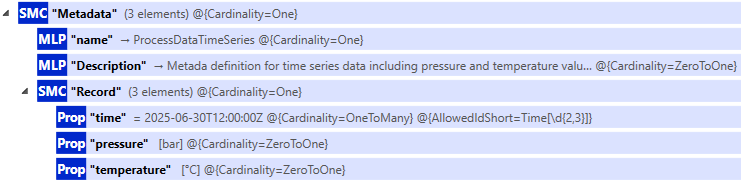
\includegraphics[width=0.88\textwidth]{Bilder/TimeSeries/MetadataTimeSeries.PNG}
    \caption{Metadaten-Konfiguration im Submodell Time Series Data}
    \label{fig:MetadataTimeSeries}
\end{figure}

Anschließend folgt die Konfiguration des LinkedSegments (siehe Abbildung \ref{fig:LinkedSegmentTimeSeries}). 
Dieses stellt die eigentliche Verbindung zu den extern gespeicherten Zeitreihendaten her.
Es enthält unter anderem den Endpunkt der InfluxDB, sowie die zugehörige Abfrage (Query), mit der die gewünschten Werte abgefragt werden können.
Zusätzlich können weitere Informationen angegeben werden, wie beispielsweise die Abtastrate (samplingRate), der Zeitraum, den das Segment abdeckt, oder ein recordCount, der angibt, wie viele Einträge innerhalb dieses Zeitraums erwartet werden.

\begin{figure}[htbp]
    \centering
    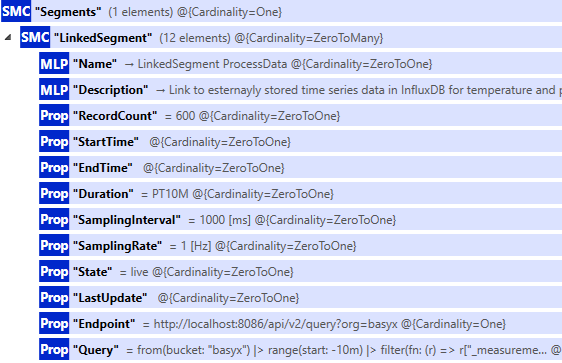
\includegraphics[width=0.86\textwidth]{Bilder/TimeSeries/LinkedSegment.PNG}
    \caption{Konfiguration des LinkedSegments im Submodell Time Series Data}
    \label{fig:LinkedSegmentTimeSeries}
\end{figure}

Zur Visualisierung der Zeitreihendaten bietet das BaSyx-System eine praktische Lösung.
Über ein entsprechendes Plugin können die im Submodell Time Series Data enthaltenen Informationen direkt in der AAS Web Ui dargestellt werden.
Die über das LinkedSegment referenzierten Zeitreihendaten lassen sich dort in verschiedenen Diagrammen visualisieren, beispielsweise als Linien- oder Balkendiagramm.
Dadurch wird eine benutzerfreundliche Darstellung der Daten ermöglicht, ohne dass diese physisch in der \acs{aas} gespeichert werden müssen.

\subsection{Anwendungsfall Digitaler Produktpass}
Im Kontext steigender Anforderungen an Nachhaltigkeit und Transparenz enlang des gesamten Produktlebenszyklus eines Assets gewinnt der \acs{dpp} zunehmend an Bedeutung.
Im Folgenden wird daher gezeigt, wie dieser mithilfe der \acs{aas} umgesetzt werden kann. 

Der Anwendungsfall orientiert sich dabei an dem von der ZVEI vorgestellten \acs{dpp40}, dessen beispielhafte Umsetzung unter anderem im Rahmen eines von ZVEI und \acs{idta} entwickelten \acs{pcf}-Showcases \cite{PCFShowcas} demonstriert wird. 
Der Fokus liegt unter anderem auf der Bereitstellung nachhaltigkeitsbezogener Informationen sowie der Umsetzung der im \acs{dpp} geforderten Zugriffsrechte für unterschiedliche Interessensgruppen.
Diese Aspekte sollen im nachfolgenden Abschnitt technisch umgesetzt werden.

Als Grundlage dient der digitale Zwilling der robocell, der im Rahmen dieses Anwendungsfalls um ein Submodell zur Abbildung des Carbon Footprints erweitert wird.
Die Umsetzung der Zugriffsrechte erfolgt mit der Eclipse BaSyx-Plattform, mit der eine rollenbasierte Zugriffskontrolle implementiert werden kann.

\subsubsection{Umsetzung mit dem Teilmodell Carbon Footprint}
Der \acs{pcf} beschreibt die Summe aller Treibhausgasemissionen, ausgedrückt in CO\textsubscript{2}-Äquivalenten, die entlang des Lebenszyklus eines Produkts entstehen \cite{PCF}. 
Zur strukturierten Erfassung dieser Werte kann das von der \acs{idta} spezifizierte Submodel Template Carbon Footprint \cite{SpezifikaitonPCF} eingesetzt werden.

Im Rahmen dieses Anwendungsfalls werden die Phasen Produktion, Material sowie die Gesamtbetrachtung (Cradle to Gate) berücksichtigt. 
Für jede Phase wird gemäß der Submodellspezifikation eine SubmodelElementCollection angelegt, die zentrale Informationen wie den CO\textsubscript{2}-Wert, die Berechnungsmethode sowie den Gültigkeitszeitraum enthält. 
Diese Sammlungen dienen als Grundlage für die spätere Aggregation der \acs{pcf}-Werte der Gesamtmaschine und werden im weiteren Verlauf dynamisch mit Werten befüllt.

Zur Ermittlung dieser Werte wird das Submodell um eine Komponentenliste erweitert, die auf die in der robocell verbauten Steuerungskomponenten verweist. 
Diese Liste bildet die Grundlage für die spätere Berechnung. 
Im Rahmen dieser Arbeit wurde exemplarisch eine Auswahl an Siemens-Komponenten betrachtet, darunter beispielsweise eine CPU sowie Ein- und Ausgangsmodule. 
Diese wurden als Typ-1-\acs{aas} zur Verfügung gestellt, wobei jede \acs{aas} ein eigenes Carbon Footprint-Submodell enthält.

Sowohl die aktualisierte \acs{aas} der robocell als auch die zugehörigen Komponenten-\acs{aas} können über die Eclipse BaSyx-Plattform bereitgestellt werden. 
Die Inhalte lassen sich so direkt über die Benutzeroberfläche der AAS Web UI einsehen. 
Zusätzlich steht ein Plugin zur Verfügung, das die Visualisierung der \acs{pcf}-Werte unterstützt.

Die dynamische Aggregation des \acs{pcf} der Gesamtmaschine erfolgt über eine externe Node.js-API, die über eine im Vue.js-basierten Plugin integrierte Schaltfläche ausgelöst wird. 
Alternativ wäre auch eine direkte Berechnung im Plugin oder über einen Microservice denkbar. 
In der vorliegenden Umsetzung liegt die gesamte Aggregationslogik jedoch serverseitig in der API.

Die API nutzt dabei die REST-Schnittstelle des Submodel Repositories der AAS Environment, um zunächst alle in der \acs{aas} der robocell hinterlegten Komponenten auszulesen. 
Diese sind jeweils über ihre globalAssetId eindeutig referenziert. 
Mithilfe des Discovery Services werden auf Basis dieser IDs die zugehörigen Komponenten-AAS identifiziert und anschließend vom AAS Repository abgerufen. 
Für jede dieser Komponenten wird geprüft, ob ein Carbon Footprint-Submodell vorhanden ist. 
Falls dies zutrifft, wird das Submodell ausgelesen und die enthaltenen Werte extrahiert.

Aus den ermittelten Einzelwerten berechnet die API schließlich die aggregierten CO\textsubscript{2}-Äquivalente für die Phasen Produktion, Material sowie Cradle to Gate. 
Die berechneten Werte werden abschließend in das Carbon Footprint-Submodell der Haupt-\acs{aas} der robocell geschrieben und stehen dort strukturiert zur Verfügung.

Die beschriebene Lösung ermöglicht es, den \acs{pcf} dynamisch auf Basis der in der Komponentenliste referenzierten Steuerungselemente zu berechnen. 
Auch wenn derzeit nur ausgewählte Komponenten berücksichtigt werden, lässt sich die Liste bei Verfügbarkeit weiterer Komponenten-\acs{aas} unkompliziert erweitern, sodass sukzessive die gesamte Maschine in die Berechnung einbezogen werden kann. 
Perspektivisch lässt sich die Berechnung zudem um weitere Lebenszyklusphasen wie Nutzung oder Entsorgung ergänzen, um eine ganzheitliche Betrachtung von der Herstellung bis zum Lebensende eines Produkts bzw. einer Maschine zu ermöglichen.

\subsubsection{Zugriffsrechte und Datensicherheit}
Das vlt zu komplex \dots
Einfach weglassen ? 
\newpage
\subsection{Anwendungsfall automatisierte Generierung von AAS}
Ziel dieses Anwendungsfalles ist es, den Prozess der automatisierten Generierung und Bereitstellung einer \acs{aas} darzustellen.
Dazu wird zunächst ein Submodel Template im Package Explorer erstellt und anschließend in ein Typ-Submodell überführt.
Dieses wird anschließend automatisiert mit Daten befüllt, in eine \acs{aas}-Instanz eingebettet und schließlich in ein Industrie 4.0-System eingebunden.

\subsubsection{Erstellen von Submodel Templates}
Das Erstellen von Submodel Templates spielt eine zentrale Rolle für den effizienten Einsatz der \acs{aas} in Industrie 4.0-Anwendungen. 
Ein einmal definiertes Template kann für beliebig viele Instanzen eines digitalen Zwillings wiederverwendet werden. 
Dadurch wird nicht nur die Konsistenz der Datenstruktur sichergestellt, sondern auch der Entwicklungsaufwand erheblich reduziert.

Grundsätzlich gibt es mehrere Möglichkeiten ein solches Template zu erstellen.
Es kann entweder vollständig neu modelliert oder von bestehenden Submodel Templates abgeleitet werden, wie es im Folgenden exemplarisch anhand des Submodells Technische Daten \cite{SpezifikaitonTechnischeDaten} gezeigt wird.
Dieses Template stellt eine standardisierte Struktur zur Beschreibung technischer Merkmale eines Produkts bereit.

Für die technische Umsetzung kann der Package Explorer eingesetzt werden.
Hierfür muss zunächst das Submodel Template Technische Daten importiert werden.
Dabei handelt es sich um ein generisches Template, das lediglich grundlegende Strukturkategorien vorgibt.
Es enthält beispielsweise SubmodelElementCollections wie Generelle Informationen, Technische Informationen oder Produktklassifikation, die allerdings noch nicht mit konkreten Eigenschaften gefüllt sind.

Auf Unternehmensebene kann dieses Template für eine bestimmte Produktgruppe mit zusätzlichen Merkmalen individualisiert werden.
So lassen sich beispielsweise spezifische Anforderungen bzw. produktspezifische Eigenschaften wie Umgebungsbedingungen oder elektrische Daten einer Maschine ergänzen.

Aus dem angepassten Template kann anschließend eine Typ-\acs{aas} erstellt werden, in die bereits konkrete allgemeingültige Merkmale einer Produktgruppe eingetragen werden.
Diese dient als Vorlage für die spätere Instanziierung konkreter digitaler Zwillinge einzelner Produkte, bei denen dann auch die produktspezifischen Werte ergänzt werden.
Zur Weiterverwendung kann das Submodell direkt im Package Explorer als JSON-Datei exportiert werden.
% Das Erstellen von Submodel Templates spielt eine wichtige Roll für den späteren Einsatz\dots
% Einmal ein Submodel template erstelllen, später für alle Insatnzen wiederverwendet werden
% Dies spart enorm an Zeit bei der Entwicklung 

% Eine Möglichkeit zur Erstellung der Templates mit dem Package Explorer
% Hierfür kann er als Expertentool eingesetzt werden
% Dort kann das strukturiert aufgebaut werden
% Das ist dann ein Template und kann anschließend mit Daten gefüllt werden.


% Beispiel technische Daten mit Abbildung

% \begin{figure}[htbp]
%     \centering
%     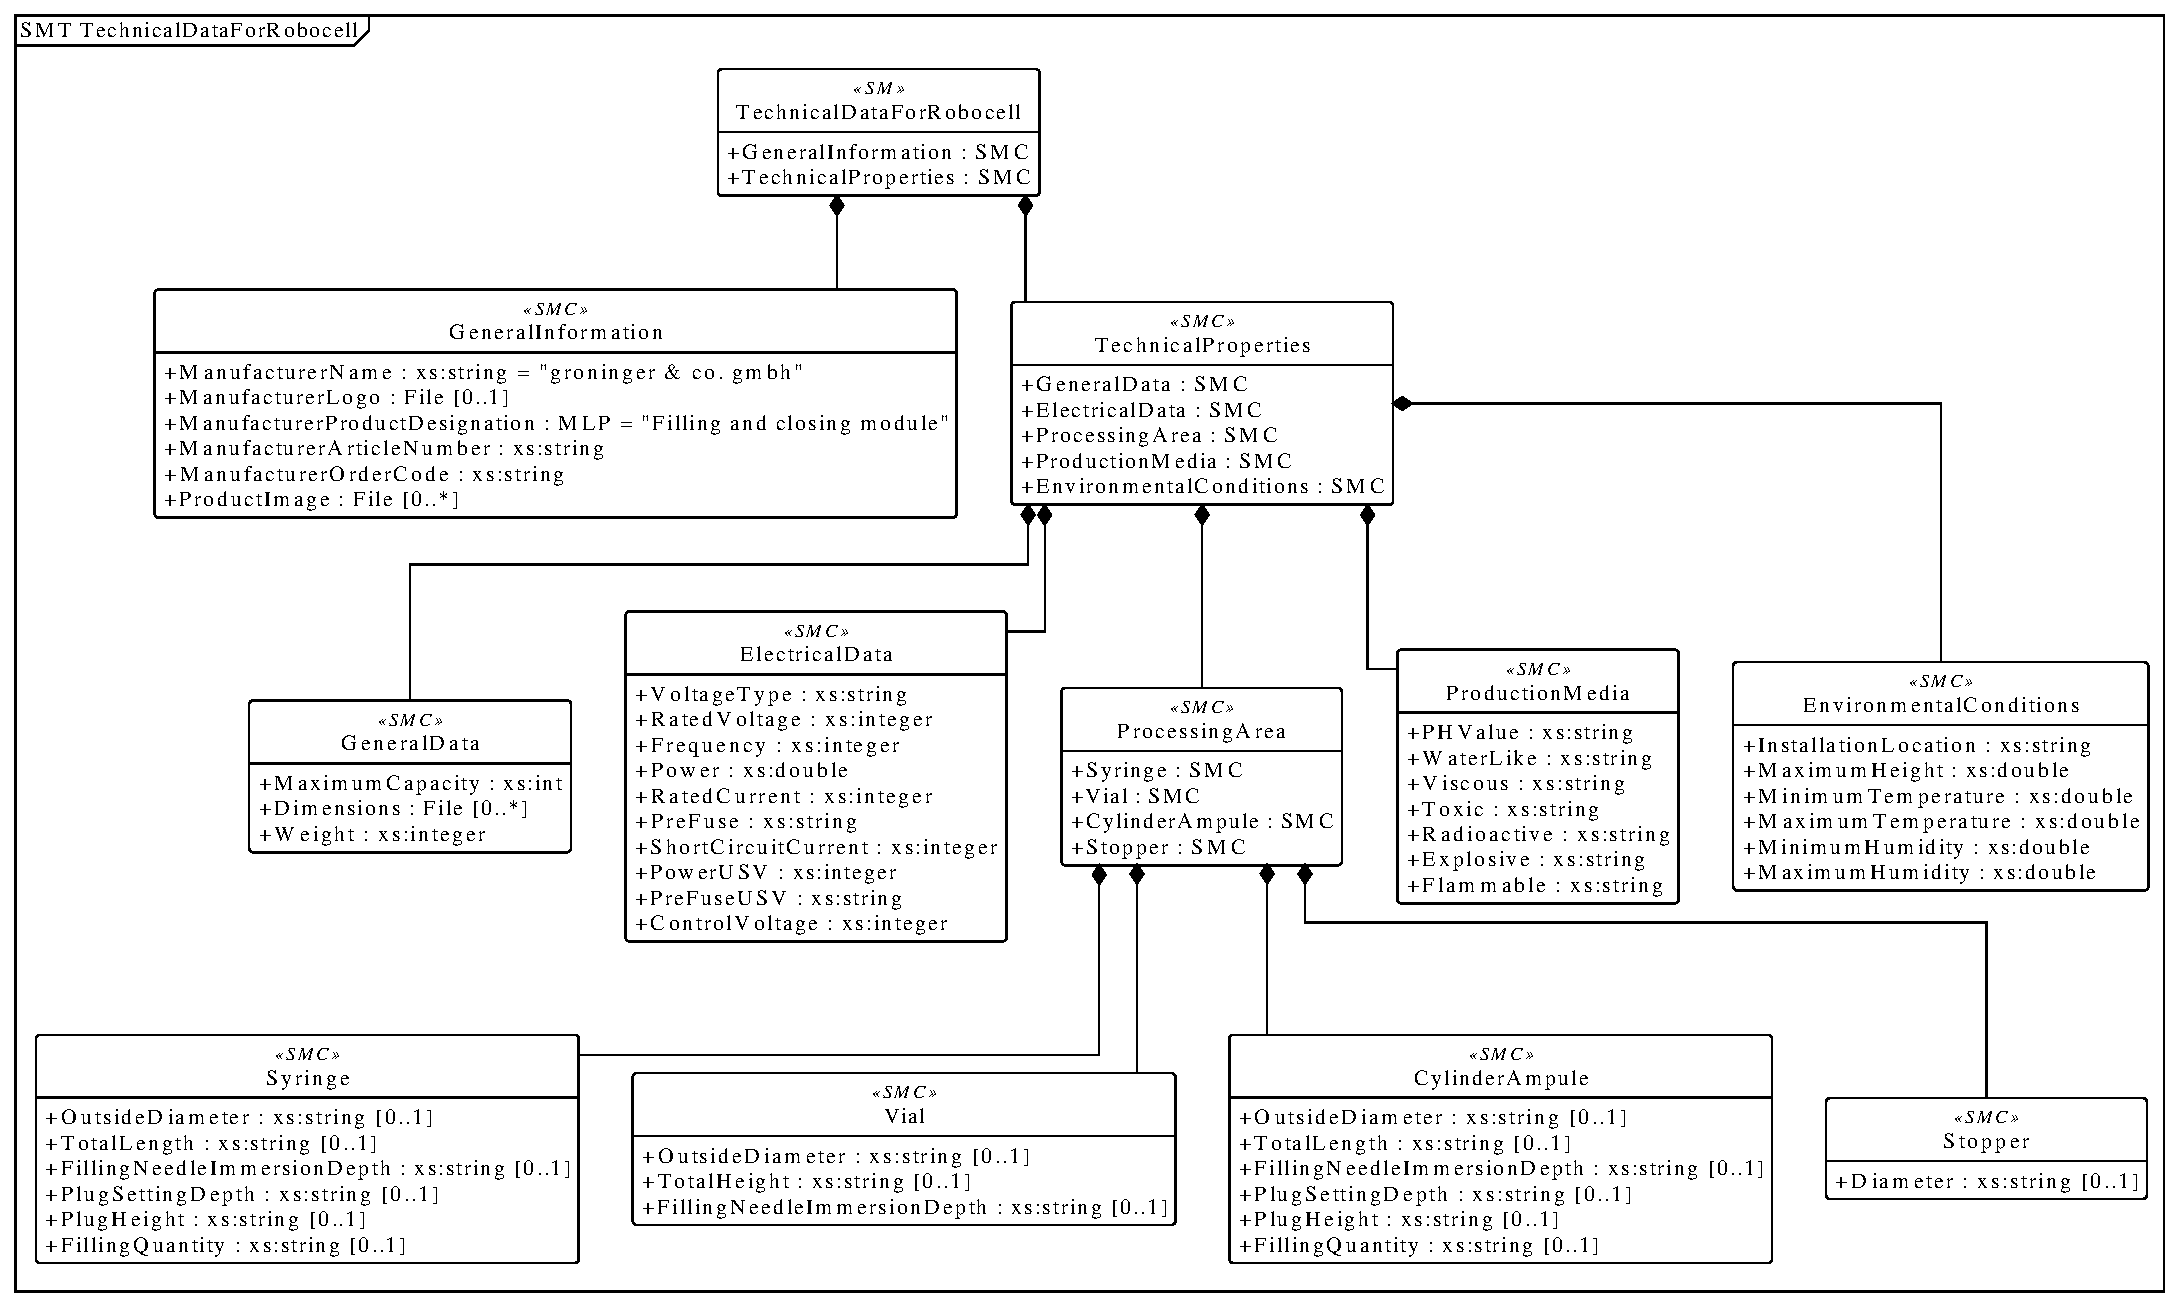
\includegraphics[width=1\textwidth]{Bilder/UML/tehcnicalDataForRobocell.pdf}
%     \caption{!!!}
%     \label{fig:!!!}
% \end{figure}

\subsubsection{Automatisiertes Befüllen mit strukturierten Daten}
Nach der Erstellung eines Typ-Submodells stellt sich die Frage, wie dieses effizient mit konkreten Informationen befüllt und anschließend in eine vollständige \acs{aas}-Instanz eingebettet werden kann.
In der Praxis liegen die hierfür benötigten Daten häufig bereits strukturiert in bestehenden Unternehmenssystemen vor, beispielsweise in \acs{plm}- oder \acs{erp}-Systemen.

Da eine direkte Anbindung solcher Systeme im Rahmen dieser Arbeit nicht möglich ist, wird das automatisierte Befüllen exemplarisch anhand vorgegebener Beispieldaten umgesetzt.
Diese enthalten technische Informationen, wie sie typischerweise in den Unternehmenssystemen vorliegen, und bilden die Grundlage für die automatisierte Erstellung des Instanz-Submodells Technische Daten.

Für die technische Umsetzung bietet sich ein Skript an, das diese Daten automatisiert in die vorgegebene Submodellstruktur überträgt und anschließend in Form einer Typ-2-\acs{aas} bereitstellt.
In diesem Projekt wird dazu die serverseitige JavaScript-Laufzeitumgebung Node.js \cite{nodejs} verwendet, da sie eine einfache Verarbeitung von JSON-Daten sowie eine unkomplizierte Kommunikation mit REST-Schnittstellen ermöglicht. 
Als Basis werden drei zentrale Komponenten benötigt:

\begin{enumerate}[noitemsep, leftmargin=*, label=\textbf{\arabic*.}]
    \item \textbf{Datenquelle:} Beispieldaten technische Produktinformationen
    \item \textbf{Submodell-Vorlage:} Struktur und Semantik des Submodells
    \item \textbf{AAS-Vorlage:} Aufbau und Struktur der \acs{aas}-Instanz
\end{enumerate}

Die Datenquelle liegt im JSON-Format vor und ist hierarchisch aufgebaut.
Sie besteht aus mehreren verschachtelten Schlüssel-Wert-Paaren.
Jeder Schlüssel dient als eindeutiger Bezeichner und entspricht einem idShort-Wert eines Submodellelements innerhalb der Submodell-Vorlage.
Diese Vorlage ist so konzipiert, dass an den relevanten Stellen Platzhalter vorhanden sind, die während der Ausführung des Skripts mit den zugehörigen Werten aus der Datenquelle befüllt werden können.

Nach dem Befüllen des Submodells mit konkreten Werten muss dieses in eine zugehörige \acs{aas}-Instanz eingebunden werden. 
Die AAS-Vorlage definiert hierfür die grundlegende Struktur der \acs{aas} in einer separaten JSON-Datei. 
Diese enthält jedoch noch keine spezifischen Identifikatoren, wie beispielsweise die eindeutige ID der \acs{aas} oder des zugehörigen Assets. 
Um diese hinzuzufügen, können während der Skriptausführung zufällige UUIDv4-Werte generiert und an den entsprechenden Stellen in die Vorlage eingefügt werden.

Im Anschluss daran gilt es, die \acs{aas} in einer Industrie-4.0-Anwendung bereitzustellen. 
Hierfür kann erneut Eclipse BaSyx genutzt werden, wobei die AAS sowie das zugehörige Submodell, analog zur in Kapitel~\ref{sec:bereitstellungAAS} beschriebenen Methode der manuellen Registrierung, über die REST-API bereitgestellt werden können.

% \subsubsection{Potenziale des KI-Einsatzes}

\subsection{Anwendungsfall KI in der Industrie 4.0}

\subsubsection{Anomaliererkennung mit maschinellem Lernen}
Datenquelle
Umsetzung mit pytorch
Modelltraining mit Autoencoder
Modell sepcihern mit onnx


Bild erst in Ergebnissse

\subsubsection{Modellverwaltung mit der \acs{aas}}

